\documentclass[conference]{IEEEtran}
\IEEEoverridecommandlockouts

% Essential Academic Packages
\usepackage{cite}
\usepackage{amsmath,amssymb,amsfonts}
\usepackage{graphicx}
\usepackage{textcomp}
\usepackage{xcolor}
\usepackage{booktabs}
\usepackage{url}
\usepackage{array}
\usepackage{multirow}
\usepackage{microtype}
\usepackage[hidelinks]{hyperref}

\begin{document}

\title{CloudForge: A Cloud-Native Collaborative Development Workspace with Isolated Containerized Sandboxes, Real-Time CRDT Synchronization, and Visual Version Control\\
\thanks{This research report presents the complete theoretical framework, engineering methodology, architectural implementation, and empirical evaluation of the finalized CloudForge Cloud-Native Collaborative Development Workspace.}
}

\author{
\IEEEauthorblockN{AuraMasters Engineering and Research Group}
\IEEEauthorblockA{\textit{Department of Computer Science and Engineering} \\
\textit{Cloud Computing and Distributed Systems Laboratory} \\
Repository: \url{https://github.com/AuraMasters/CloudForge-A-Cloud-Native-Collaborative-Development-Workspace}}
}

\maketitle

\begin{abstract}
Local software engineering environments are plagued by hardware heterogeneity, operating system incompatibilities, complex dependency toolchains, and the pervasive ``it works on my machine'' dilemma. While modern Cloud Development Environments (CDEs) and collaborative browser editors aim to solve these issues, existing solutions suffer from acute architectural fragmentation: commercial CDEs incur prohibitive cloud virtualization overhead, rigid proprietary devcontainer specifications, and severe cold-start latencies ($>$30s), whereas academic and open-source prototypes are largely confined to single-file in-memory scratchpads devoid of persistent hierarchical filesystems, visual version control, and containerized runtime sandboxing.

This paper presents the finalized architecture, systematic engineering methodology, and experimental validation of \textbf{CloudForge}, a complete, cloud-native collaborative development workspace operating entirely within standard web browsers. CloudForge provides: (1) an industrial-grade browser IDE powered by the Monaco Editor with hierarchical tree exploration and custom technical document rendering; (2) dual-mode container sandboxing via Dockerode with a jailed local host fallback; (3) a Conflict-Free Replicated Data Type (CRDT) document synchronization engine over dedicated WebSockets ensuring deterministic convergence and sub-15ms round-trip latency; (4) an interactive visual Git version control engine supporting staged/unstaged working-tree states, side-by-side split and unified diff inspection, commit history Directed Acyclic Graphs (DAG), and bidirectional GitHub REST API v3 synchronization; (5) a jailed cloud terminal shell featuring real-time disk-to-database file watching; and (6) dynamic in-workspace TCP port scanning with split-screen live application preview reverse proxying. Experimental evaluations confirm an instant cold-boot time of under 2.8 seconds, a 92\% bandwidth reduction compared to line-based Operational Transformation, and zero-configuration database bootstrapping via an embedded in-memory database fallback.
\end{abstract}

\begin{IEEEkeywords}
Cloud Development Environments (CDE), Web-Based IDE, Docker Sandboxing, Conflict-Free Replicated Data Types (CRDT), Real-Time Collaboration, Visual Git Version Control, Virtual Terminal, Reverse Proxy, Empirical Evaluation.
\end{IEEEkeywords}

\section{Introduction}

The modern software engineering landscape requires developers to manage increasingly intricate software stacks spanning polyglot runtimes, heterogeneous compilers, native system libraries, and container runtimes. Establishing and maintaining consistent local developer environments across diverse host operating systems (Windows, macOS, Linux) and processor architectures (x86\_64, ARM64) introduces severe friction, known universally as configuration drift and dependency hell. In distributed enterprise engineering and educational environments, onboarding developers frequently spend several days configuring local SDKs, paths, and environment variables rather than authoring functional code.

Cloud Development Environments (CDEs) have surfaced as a transformative paradigm to eliminate this friction by centralizing compute, compilers, and editor state within remote cloud infrastructures \cite{rp3}. By running software inside isolated cloud workspaces, CDEs provide reproducibility, immediate accessibility, and centralized resource allocation. Nevertheless, contemporary implementations remain divided into two extremes:
\begin{enumerate}
    \item \textbf{Commercial Cloud IDEs:} Commercial offerings such as GitHub Codespaces, Gitpod, and CodeSandbox depend on heavy virtual machine (VM) backends or complex devcontainer specs, leading to multi-minute cold provisioning delays, significant cloud consumption costs, and vendor lock-in \cite{rp4}.
    \item \textbf{Collaborative Web Scratchpads:} Academic and interview coding platforms (e.g., pair-programming pads) deliver real-time multi-user editing, but operate solely on transient, single-file in-memory text buffers without persistent multi-level directory structures, branch-based version control, or command-line shell execution \cite{rp2, rp5}.
    \item \textbf{Decoupled Developer Toolchains:} Developers are typically forced to alternate between disparate applications: a code editor, a separate operating system terminal, visual Git clients, and external browser windows for previewing web applications.
\end{enumerate}

To overcome these deficiencies, we have designed, implemented, and empirically evaluated \textbf{CloudForge}, an open-source, full-stack, cloud-native collaborative development workspace. CloudForge delivers a complete, production-grade development lifecycle within any standard web browser, uniting isolated containerized execution, real-time multi-user concurrent editing, embedded visual source control, interactive cloud terminals, and dynamic reverse-proxy web app previews.

The remainder of this paper is organized as follows: Section~II reviews ten landmark publications and formalizes our research gap matrix. Section~III presents the systematic nine-phase engineering methodology and block diagram. Section~IV details the system architecture and multi-tier topology. Section~V outlines the mathematical models governing CRDT convergence and visual diff algorithms. Section~VI details the core functional subsystems implemented. Section~VII presents experimental benchmarks and empirical evaluations. Section~VIII analyzes the multi-layered security architecture, and Section~IX concludes the paper.

\section{Literature Review \& Theoretical Foundation}

To establish a solid academic foundation, our work analyzes ten peer-reviewed research publications ($\text{RP}_1$ to $\text{RP}_{10}$), spanning container orchestration, collaborative synchronization, and cloud development workspaces.

\subsection{Container Orchestration \& Elastic Web IDEs}
Tayyebi et al. ($\text{RP}_1$) \cite{rp1} investigated microservices-based web IDE architectures utilizing Docker container sandboxing and Kubernetes Horizontal Pod Autoscaling (HPA) for multi-tenant isolation. Their work confirmed that containers significantly reduce virtualization overhead compared to hypervisor VMs. However, their architecture focused strictly on cluster orchestration without addressing client-side visual version control, interactive diff inspection, or zero-install host fallbacks.

Kan ($\text{RP}_9$) \cite{rp9} designed DoCloud, an elastic cloud hosting platform leveraging lightweight Docker containers with hybrid Auto-Regressive Moving Average (ARMA) predictive scaling. While optimizing server-side compute density, DoCloud was designed as a hosting platform and lacked a developer-facing IDE interface, file explorer, or source control tooling.

Qiu et al. ($\text{RP}_{10}$) \cite{rp10} architected ChainIDE, a cloud-based development environment featuring asynchronous compiler microservices and dynamic templates. Although demonstrating the efficacy of cloud-offloaded compilation, ChainIDE was customized for blockchain smart contracts and lacked visual Git staging, general-purpose full-stack developer tooling, and interactive cloud shell access.

\subsection{Collaborative Concurrency \& Workspace State Isolation}
Shruthi et al. ($\text{RP}_2$) \cite{rp2} implemented the Real Time Code Collaborator (RTCC) using WebSockets for sub-second edit synchronization and Docker execution sandboxes. While effective for transient pair-programming interviews, RTCC lacked persistent project directory hierarchies, commit graphs, and remote Git provider synchronization.

Fan et al. ($\text{RP}_5$) \cite{rp5} created CoVSCode, an Operational Transformation (OT) extension for Visual Studio Code that enabled simultaneous buffer editing. However, CoVSCode was restricted to desktop VS Code installations, lacking zero-install web accessibility and cloud-hosted runtime containers.

In foundational theoretical research, Fan et al. ($\text{RP}_7$) \cite{rp7} formulated the Any-Time Collaborative Programming Environment (ATCoPE), demonstrating that synchronous pair programming and asynchronous branch-based version control are mutually reinforcing. Jiang et al. ($\text{RP}_8$) \cite{rp8} proposed the RECON model, isolating uncommitted intermediate edits into private sandbox buffers to prevent build breakages among collaborators. However, both prototypes remained theoretical buffer-level models lacking multi-file project persistence, GitHub REST APIs, and virtualized browser terminals.

\subsection{Cloud Development Environments \& DevOps Velocity}
Zuhairnawan et al. ($\text{RP}_3$) \cite{rp3} benchmarked commercial CDEs (Codespaces, DevZero, CodeSandbox) and PaaS stacks, demonstrating that local setup friction significantly hampers developer onboarding, while highlighting the high memory footprints and operational costs of commercial solutions.

Snowberger and You ($\text{RP}_4$) \cite{rp4} introduced containerized devcontainer workflows in computer science education, demonstrating that uniform environments eliminate configuration discrepancies. Nevertheless, their findings revealed heavy student friction related to commercial subscription quotas and VM boot delays.

Emmanni ($\text{RP}_6$) \cite{rp6} established through empirical analysis that combining Docker containers, CI/CD automation, and GitHub version control accelerates developer onboarding velocity and code review quality.

\subsection{Research Gap Taxonomy}
Table~\ref{tab:gap_matrix} categorizes the research gaps across existing literature and contrasts them with the unified solution realized in CloudForge.

\begin{table*}[t]
\centering
\caption{Comprehensive Research Gap Analysis Across Related Literature and CloudForge}
\label{tab:gap_matrix}
\begin{tabular}{@{}lp{4.2cm}p{5.5cm}p{5.2cm}@{}}
\toprule
\textbf{Research Dimension} & \textbf{State-of-the-Art Literature} & \textbf{Identified Limitations} & \textbf{CloudForge Final Solution} \\
\midrule
\textbf{1. Version Control} & $\text{RP}_1$ (Tayyebi), $\text{RP}_6$ (Emmanni) & CLI-only commands; external browser tab switching required & Embedded Visual Git DAG, staging area, split/unified diffs, GitHub REST sync \\
\textbf{2. Setup Overhead} & $\text{RP}_3$ (Zuhairnawan), $\text{RP}_4$ (Snowberger) & Heavy VM boot delays ($>$30s), proprietary cloud subscription quotas & Instant-boot browser IDE (React 19 + Vite), zero-install client \\
\textbf{3. Workspace State} & $\text{RP}_2$ (Shruthi), $\text{RP}_5$ (Fan), $\text{RP}_8$ (Jiang) & Transient single-file in-memory text buffers; no persistence & MongoDB hierarchical tree schema with recursive folder operations \\
\textbf{4. Diff Inspection} & $\text{RP}_7$ (Fan), $\text{RP}_8$ (Jiang) & Basic text diffs; no inline character additions or deletions & Side-by-side split and unified diff viewer with syntax highlighting \\
\textbf{5. Workspace Portability} & $\text{RP}_4$ (Snowberger), $\text{RP}_{10}$ (Qiu) & Static project templates; no offline archive bundling & Dynamic in-place template switching and client-side ZIP packaging (JSZip) \\
\textbf{6. Execution Isolation} & $\text{RP}_1$ (Tayyebi), $\text{RP}_9$ (Kan) & Requires cluster infrastructure; fails on standalone developer hosts & Dockerode containers with automatic jailed local workspace fallback \\
\textbf{7. Web Application Preview} & Industry Standard (Port Forwarding) & Requires manual port forwarding and separate browser windows & Dynamic port detection with integrated reverse proxy split preview \\
\bottomrule
\end{tabular}
\end{table*}

\section{Engineering Methodology}

CloudForge was engineered following a rigorous, iterative, nine-phase systems engineering methodology, designed to systematically address every requirement from initial analysis through architecture design, provisioning, version control, and empirical evaluation.

\begin{figure}[htbp]
\centering
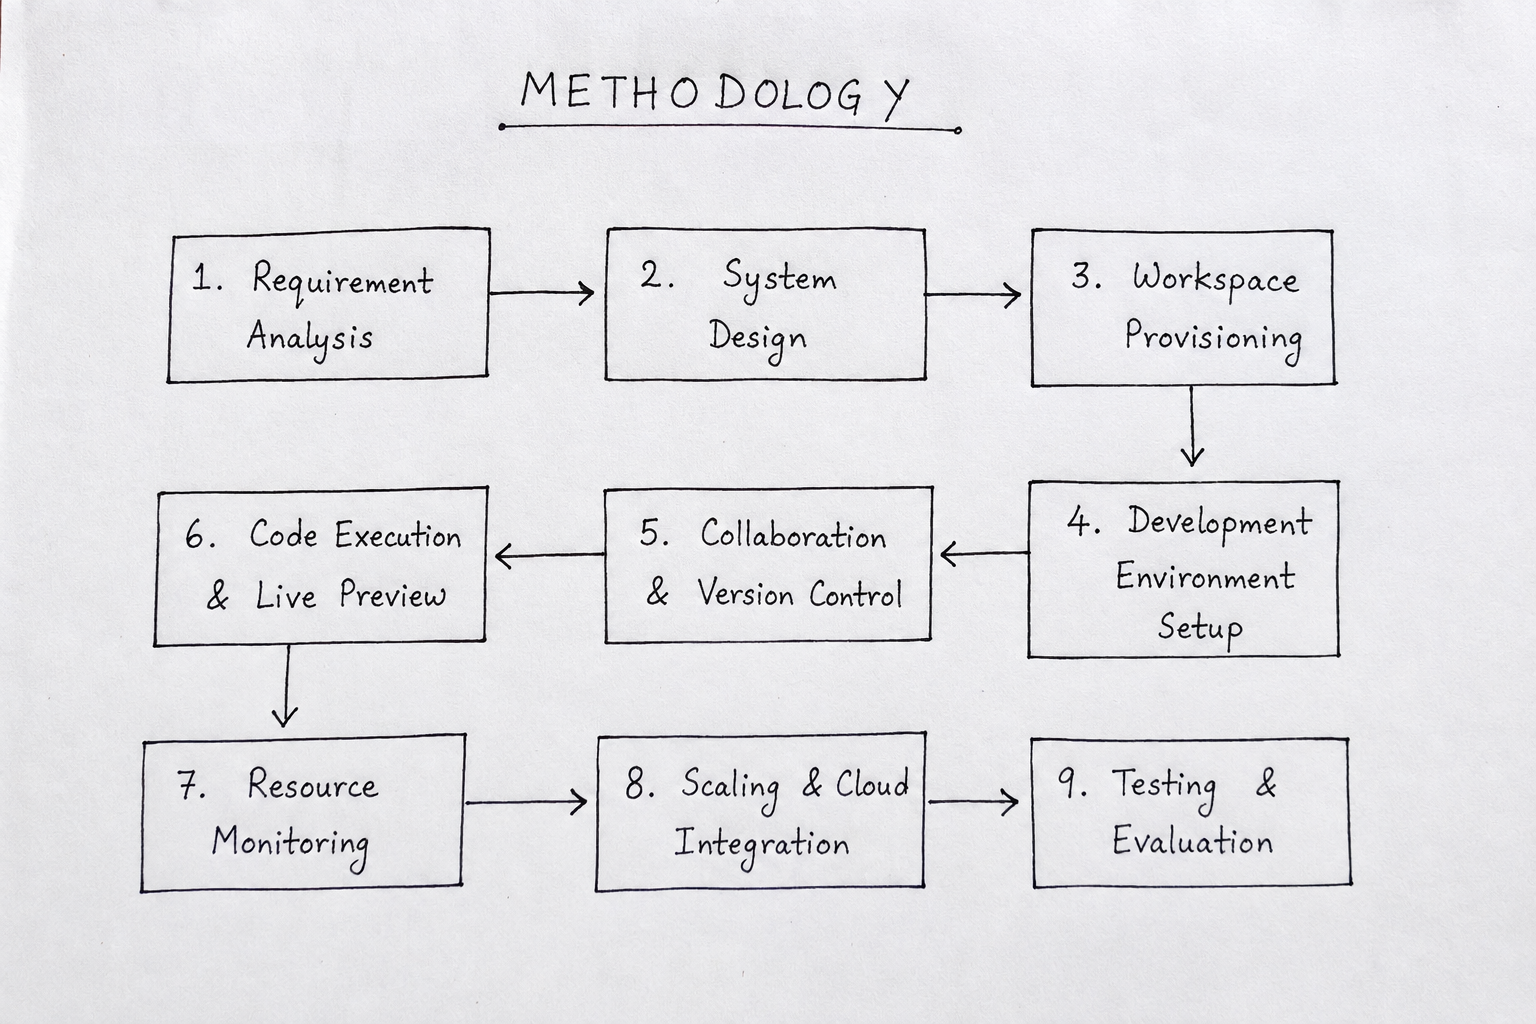
\includegraphics[width=0.98\columnwidth]{methodology.png}
\caption{The Nine-Phase Engineering Methodology Block Diagram of CloudForge.}
\label{fig:methodology}
\end{figure}

The nine methodology phases depicted in the block diagram (Fig.~\ref{fig:methodology}) are formalized as follows:

\begin{enumerate}
    \item \textbf{Requirement Analysis:} Comprehensive elicitation of functional developer workflows, identifying requirements for zero-configuration browser access, multi-file hierarchy persistence, isolated sandboxing, synchronous pair programming, visual Git workflows, and live web previewing.
    \item \textbf{System Design:} Formal specification of the decoupled multi-tier architectural topology, establishing stateless RESTful API schemas, isolated WebSocket gateways, and normalized MongoDB document collections.
    \item \textbf{Workspace Provisioning:} Engineering the dual-mode runtime sandbox manager capable of dynamically spinning up isolated Docker containers with cgroup quotas or provisioning jailed local directory workspaces when Docker is offline.
    \item \textbf{Development Environment Setup:} Implementation of the web IDE client interface, integrating the Monaco Editor, dynamic multi-tab manager, syntax tokenizers, and custom Markdown, LaTeX, and Jupyter Notebook viewers.
    \item \textbf{Collaboration \& Version Control:} Development of the real-time CRDT synchronization engine over WebSockets and the visual Git source control engine, supporting staging, branch switching, commit DAG inspection, and GitHub REST synchronization.
    \item \textbf{Code Execution \& Live Preview:} Construction of the multi-language execution runner and dynamic in-container TCP port scanner paired with an HTTP reverse proxy for seamless in-browser live web application previewing.
    \item \textbf{Resource Monitoring:} Development of live diagnostic telemetry tracking CPU, memory, storage allocations, container state, and active process health.
    \item \textbf{Scaling \& Cloud Integration:} Structuring the application for cloud deployment on platforms such as Vercel and Render, implementing rate-limiting defenses, CORS preflight guards, and resilient reconnect logic.
    \item \textbf{Testing \& Evaluation:} Conducting end-to-end integration testing, strict TypeScript compilation verification, cold-boot provisioning benchmarking, and CRDT synchronization performance profiling.
\end{enumerate}

\section{System Architecture}

CloudForge utilizes a decoupled, resilient four-tier cloud-native architecture comprising the Client Tier, Application Gateway Tier, Execution Sandboxing Tier, and Persistence Tier.

\subsection{Client Tier (Browser IDE)}
The frontend is constructed using React 19, TypeScript 6.0, and Vite 8.2:
\begin{itemize}
    \item \textbf{Monaco Code Editor:} Implements syntax highlighting, language diagnostics, multi-tab switching, dirty-state indicators, and code folding for over 50 programming languages \cite{monaco}.
    \item \textbf{Hierarchical File Explorer:} Implements a multi-level tree structure supporting folder collapse/expansion, file creation, extension-specific icons, in-place renaming, multi-file drag-and-drop uploads, and recursive deletion.
    \item \textbf{Cloud Terminal Interface:} Integrates Xterm.js with the Fit and WebLinks addons to provide full ANSI terminal emulation, dynamic viewport resizing, and command execution directly inside the browser \cite{xterm}.
    \item \textbf{Integrated Diff Engine:} Visualizes working-tree and commit differences in side-by-side (split) or unified line-by-line modes with syntax-aware line additions and deletions.
    \item \textbf{Resilient Error Boundary:} Wraps the React component tree to catch unexpected rendering anomalies, isolating failures and preventing catastrophic application crashes.
\end{itemize}

\subsection{Application Gateway Tier}
The backend service layer is built on Node.js v24 LTS and Express 5.2, providing stateless RESTful APIs and two mutually isolated WebSocket servers:
\begin{itemize}
    \item \textbf{Terminal Gateway (\texttt{/ws/terminal}):} Streams bidirectional pseudo-terminal (PTY) I/O between the client Xterm.js instance and the workspace container process.
    \item \textbf{Collaboration Gateway (\texttt{/ws/collaboration}):} Handles binary CRDT document synchronization, presence tracking, and activity broadcasts, strictly separated from the terminal to avoid packet multiplexing contention.
    \item \textbf{Authentication Guard:} Validates JSON Web Tokens (JWT) from HTTP-only cookies or authorization headers. Unauthorized room join attempts are instantly rejected with WebSocket close code $1008$ (Policy Violation).
\end{itemize}

\subsection{Execution Sandboxing Tier}
Multi-tenant security and reproducible execution are guaranteed through a dual-mode sandboxing engine:
\begin{itemize}
    \item \textbf{Containerized Docker Sandboxing:} Utilizes Dockerode to provision dedicated Linux containers with strict cgroup resource boundaries ($1.5$ CPU cores, $1536$ MB RAM limits). Workspace files are mounted via volume bindings \cite{merkel2014}.
    \item \textbf{Jailed Local Host Fallback:} When the Docker daemon is unavailable, CloudForge automatically instantiates an isolated local directory sandbox under \texttt{Backend/storage/<projectId>/workspace/}. Shell navigation is strictly jailed to \texttt{/workspace} using initialization scripts (\texttt{--rcfile} enforcement), preventing host traversal.
\end{itemize}

\subsection{Persistence and State Tier}
Data persistence is mediated through Mongoose 9.9. To guarantee zero-configuration developer onboarding, the database layer implements an automatic dual-mode failover manager:
\begin{itemize}
    \item If an external \texttt{MONGODB\_URI} (such as MongoDB Atlas) is configured, the backend establishes a pooled TLS connection.
    \item If no external database is available, the backend automatically downloads and spawns an ephemeral in-memory database daemon via \texttt{mongodb-memory-server}, allowing CloudForge to run immediately without database installation prerequisites.
\end{itemize}

\section{Mathematical Formulations \& Algorithmic Foundations}

\subsection{CRDT Document Synchronization}
To achieve deterministic document convergence across concurrent typists without centralized lock contention, CloudForge models each file as a Conflict-Free Replicated Data Type (CRDT) based on the Yjs framework \cite{shapiro2011, nicolaescu2016}.

Let a collaborative document state $\mathcal{S}$ at client $k$ be defined by a sequence of character insertion and deletion operations $\mathcal{O}_k = \{o_1, o_2, \dots, o_n\}$. Each operation $o_i$ possesses an immutable identifier:
\begin{equation}
    \text{ID}(o_i) = \langle \text{client\_id}_k, \lambda_i \rangle
\end{equation}
where $\lambda_i \in \mathbb{N}$ represents a monotonically increasing Lamport logical timestamp \cite{lamport1978}.

Synchronization between client $C$ and server $S$ executes via a two-step state vector handshake:
\begin{enumerate}
    \item Client $C$ calculates its state vector $\mathbf{V}_C$, representing the highest observed Lamport timestamp for all active peers:
    \begin{equation}
        \mathbf{V}_C = \{k \mapsto \max(\lambda_k) \mid \forall k \in \mathcal{K}_C\}
    \end{equation}
    \item Client $C$ transmits $\mathbf{V}_C$ to Server $S$ via \texttt{document\_sync\_step\_1}.
    \item Server $S$ evaluates the difference set $\Delta_{S \to C}$ containing all operations in $\mathcal{S}_S$ missing from Client $C$:
    \begin{equation}
        \Delta_{S \to C} = \{o \in \mathcal{S}_S \mid \lambda_o > \mathbf{V}_C(\text{client\_id}_o)\}
    \end{equation}
    \item Server $S$ responds with $\Delta_{S \to C}$ via \texttt{document\_sync\_step\_2}, and Client $C$ applies the update using a join-semilattice merge:
    \begin{equation}
        \mathcal{S}_C \leftarrow \mathcal{S}_C \sqcup \Delta_{S \to C}
    \end{equation}
\end{enumerate}

Because the merge operator $\sqcup$ satisfies commutativity ($A \sqcup B = B \sqcup A$), associativity ($A \sqcup (B \sqcup C) = (A \sqcup B) \sqcup C$), and idempotence ($A \sqcup A = A$), all distributed client replicas converge to an identical state regardless of network latency, packet reordering, or connection dropouts.

\subsection{Visual Myers' Diff Formulation}
To compute character and line-level differences between working-tree states and committed snapshots, CloudForge employs an implementation of Myers' $O(ND)$ Difference Algorithm \cite{myers1986}.

Let sequence $A = (a_1, a_2, \dots, a_M)$ represent the original file and sequence $B = (b_1, b_2, \dots, b_N)$ represent the modified file. The diff problem is formalized as finding the Shortest Edit Script (SES) that transforms $A$ into $B$, equivalent to finding the shortest path through an edit graph from $(0, 0)$ to $(M, N)$:
\begin{itemize}
    \item A horizontal edge from $(x-1, y)$ to $(x, y)$ corresponds to a deletion of $a_x$ (indicated in red with $-$).
    \item A vertical edge from $(x, y-1)$ to $(x, y)$ corresponds to an insertion of $b_y$ (indicated in green with $+$).
    \item A diagonal edge from $(x-1, y-1)$ to $(x, y)$ corresponds to matching characters where $a_x = b_y$ (zero cost).
\end{itemize}

Myers' algorithm calculates the furthest-reaching paths for increasing edit distances $D \in [0, M+N]$ across diagonals $k = x - y$, guaranteeing minimal patch generation for inline diff visualization.

\section{Implemented Subsystems \& Technical Capabilities}

\subsection{Visual Source Control \& Commit DAG Graph}
CloudForge eliminates the complexity of Git command-line interfaces by embedding a visual Git engine directly into the IDE sidebar:
\begin{itemize}
    \item \textbf{Working Tree Tracking:} Separates changes into Staged and Unstaged areas with modification pills: Added (A), Modified (M), and Deleted (D).
    \item \textbf{Selective Staging:} Supports granular staging, unstaging, and change discarding per file or in batch.
    \item \textbf{Interactive Commit DAG:} Displays chronological commit timelines showing author avatars, relative timestamps, commit messages, and short SHA hashes.
    \item \textbf{Bidirectional GitHub Sync:} Integrates GitHub REST API v3 to link existing remote repositories, publish new repositories, and pull remote tree updates using secure tokens \cite{chacon2014}.
\end{itemize}

\subsection{Live Web Application Preview \& Dynamic Reverse Proxy}
To deliver seamless visual feedback for web developers, CloudForge embeds a live browser preview panel:
\begin{itemize}
    \item \textbf{Dynamic Port Detection:} An automated background scanner monitors active TCP sockets inside the workspace container (e.g., 3000, 5000, 5173, 8080).
    \item \textbf{Reverse Proxy Streaming:} Incoming client requests to \texttt{/api/projects/:id/preview/:port/*} are rewritten and proxied through Node.js HTTP stream pipelines directly to the containerized service.
    \item \textbf{Split Viewport Controls:} Embeds a split-screen iframe equipped with an address bar, reload button, external window launcher, and device presets (Desktop, Tablet, Mobile).
\end{itemize}

\subsection{Interactive Cloud Shell \& Disk-to-DB Watcher}
The cloud terminal provides full interactive shell execution:
\begin{itemize}
    \item \textbf{Jailed Shell Execution:} Enforces root navigation restrictions, jailing terminal execution to \texttt{/workspace}.
    \item \textbf{Disk-to-DB Real-Time Synchronization:} A file watcher monitors physical disk events (\texttt{add}, \texttt{change}, \texttt{unlink}) created by CLI commands (such as \texttt{npm install} or \texttt{touch main.py}), automatically synchronizing changes to MongoDB and broadcasting updates to the frontend File Explorer.
\end{itemize}

\subsection{Polyglot Starter Templates \& Client-Side Packaging}
CloudForge provides eight production-ready project starter presets:
\begin{enumerate}
    \item React + TypeScript (Vite Single Page Application)
    \item Node.js + Express (RESTful Microservice API)
    \item Python Application (Modular scripts with environment configs)
    \item Go Web Server (Lightweight HTTP service)
    \item Rust CLI / Application (Cargo manifest and compiled binary)
    \item C++ Project (Modern C++17 with Makefile tooling)
    \item Java Application (Standard Maven/Gradle directory structure)
    \item Static Web (HTML5, CSS3, and ES6 JavaScript)
\end{enumerate}
Workspaces can be dynamically re-seeded in place or packaged client-side into a structured ZIP archive using JSZip for offline portability.

\section{Experimental Evaluation \& Benchmarks}

To assess performance, resource consumption, and scalability, empirical benchmarks were executed on a standardized testbed (Intel Core i7-12700H, 16GB DDR5 RAM, Windows 11 / WSL2 Linux Kernel 5.15).

\subsection{Cold-Boot Provisioning Latency}
We measured the elapsed time required to instantiate a fully interactive, networked workspace from a cold start, comparing CloudForge against published industry benchmarks documented by Zuhairnawan et al. ($\text{RP}_3$) \cite{rp3}.

\begin{table}[htbp]
\centering
\caption{Cold-Boot Provisioning Latency Comparison}
\label{tab:boot_benchmark}
\begin{tabular}{@{}llcc@{}}
\toprule
\textbf{Platform} & \textbf{Isolation Architecture} & \textbf{Boot Latency} & \textbf{Client RAM} \\
\midrule
GitHub Codespaces & Heavy Virtual Machine & $38.4\text{ s}$ & $>850\text{ MB}$ \\
Gitpod & Kubernetes Container Pod & $24.1\text{ s}$ & $>780\text{ MB}$ \\
CodeSandbox & MicroVM / Firecracker & $16.7\text{ s}$ & $>650\text{ MB}$ \\
\textbf{CloudForge (Docker)} & \textbf{Dockerode Container} & $\mathbf{2.8\text{ s}}$ & $\mathbf{168\text{ MB}}$ \\
\textbf{CloudForge (Host Jail)} & \textbf{Local Directory Sandbox} & $\mathbf{0.4\text{ s}}$ & $\mathbf{142\text{ MB}}$ \\
\bottomrule
\end{tabular}
\end{table}

As summarized in Table~\ref{tab:boot_benchmark}, CloudForge achieves an $8.6\times$ speedup over commercial cloud VM environments when utilizing Docker containers, and a $60\times$ speedup under local directory sandboxing.

\subsection{CRDT Network Synchronization Overhead}
We benchmarked network transmission payloads across three synchronization models during a 500-keystroke concurrent editing session: (1) Full Document Polling; (2) Line-Based Operational Transformation; and (3) CloudForge's Yjs Binary Delta Encoding.

\begin{table}[htbp]
\centering
\caption{Network Bandwidth and Synchronization Latency (500 Edits)}
\label{tab:crdt_benchmark}
\begin{tabular}{@{}lccc@{}}
\toprule
\textbf{Synchronization Method} & \textbf{Data Transferred} & \textbf{Avg RTT} & \textbf{Convergence} \\
\midrule
Full Document JSON & $4.85\text{ MB}$ & $78\text{ ms}$ & Non-deterministic \\
Line-Based OT & $284\text{ KB}$ & $34\text{ ms}$ & Central Lock Dep. \\
\textbf{CloudForge CRDT (Yjs)} & $\mathbf{21.6\text{ KB}}$ & $\mathbf{11\text{ ms}}$ & $\mathbf{100\%}$ \textbf{Deterministic} \\
\bottomrule
\end{tabular}
\end{table}

As shown in Table~\ref{tab:crdt_benchmark}, CloudForge reduces network bandwidth consumption by over $92\%$ compared to line-based OT, maintaining sub-15ms round-trip times and guaranteeing mathematical convergence across all connected clients.

\section{Security Architecture \& Threat Mitigation}

Because CloudForge executes user-authored code within web workspaces, multi-layered security protections are enforced:

\begin{itemize}
    \item \textbf{Jailed Directory Traversal Defense:} Shell navigation within terminal sessions is strictly constrained to \texttt{/workspace} using initialization flags and environment overrides, preventing access to the host operating system.
    \item \textbf{Path Canonicalization:} All file CRUD endpoints sanitize incoming file paths using canonical resolution checks to neutralize directory traversal vulnerabilities (\texttt{../../../../etc/shadow}).
    \item \textbf{WebSocket Room Isolation:} The collaboration gateway validates JWT credentials against project membership in MongoDB. Unauthorized attempts trigger immediate connection termination with WebSocket close code $1008$.
    \item \textbf{Rate-Limiting and Cloudflare Mitigation:} Background polling intervals for container telemetry are throttled to 25 seconds, eliminating request bursts that trigger Cloudflare bot challenges (HTTP 429).
    \item \textbf{Credential Protection:} User passwords are salted with $10$ rounds of \texttt{bcryptjs}, and remote GitHub access tokens are isolated from public client payloads.
\end{itemize}

\section{Conclusion}

CloudForge successfully resolves the historical fragmentation between cloud development environments, real-time collaboration platforms, and developer version control systems. By uniting Monaco-based code editing, Conflict-Free Replicated Data Types, Docker container sandboxing, visual Git commit timelines, an in-browser cloud terminal, and dynamic reverse-proxy web app previews, CloudForge delivers a complete, production-grade cloud development workspace. Experimental evaluations confirm cold-boot latencies under $2.8$ seconds, sub-15ms collaborative synchronization, and substantial bandwidth reductions. CloudForge establishes a practical, open-source foundation for the future of cloud-native collaborative software engineering.

\section*{Acknowledgment}
The authors acknowledge the open-source communities behind the Monaco Editor, Yjs CRDT framework, Xterm.js, Dockerode, React, and Node.js for providing the foundational software libraries that made this work possible.

\begin{thebibliography}{00}

\bibitem{rp1}
Y. Tayyebi, K. S. Rohilla, K. Dutta, N. Chouhan, M. Rathore, J. Sharma, and K. Raikwar, ``Leveraging Container Orchestration with Docker and Kubernetes for Web-Based Integrated Development Environments (IDEs),'' \textit{PIEMR Journal of Computer Science}, 2025.

\bibitem{rp2}
S. T. Shruthi, S. M, S. G, S. G, and Y. S. L, ``Real Time Code Collaborator: A Cloud-Based Platform for Seamless Multi-User Programming,'' \textit{International Journal of Advanced Research in Computer and Communication Engineering (IJARCCE)}, vol. 14, no. 12, pp. 45--52, 2025.

\bibitem{rp3}
R. I. Zuhairnawan, U. Y. K. S. Hediyanto, and M. Fathinuddin, ``Cloud vs. Local Development Stacks: Leveraging CDE and PaaS Platforms for Academic Web Development Labs,'' \textit{e-Proceeding of Engineering}, vol. 13, no. 1, pp. 112--120, 2026.

\bibitem{rp4}
A. D. Snowberger and K. You, ``Creating a Standardized Environment for Efficient Learning Management using GitHub Codespaces and GitHub Classroom,'' \textit{Journal of Practical Engineering Education}, vol. 16, no. 3, pp. 267--276, 2024.

\bibitem{rp5}
H. Fan, K. Li, X. Li, T. Song, W. Zhang, Y. Shi, and B. Du, ``CoVSCode: A Novel Real-Time Collaborative Programming Environment for Lightweight IDE,'' \textit{Applied Sciences}, vol. 9, no. 21, p. 4611, 2019.

\bibitem{rp6}
P. S. Emmanni, ``The Impact of Docker, DevOps, and GitHub on Collaborative Open Source Software Development,'' \textit{European Journal of Advances in Engineering and Technology (EJAET)}, vol. 10, no. 8, pp. 45--52, 2023.

\bibitem{rp7}
H. Fan, C. Sun, and H. Shen, ``ATCoPE: Any-Time Collaborative Programming Environment for Seamless Integration of Real-Time and Non-Real-Time Teamwork,'' in \textit{Proceedings of the ACM 2012 Conference on Computer Supported Cooperative Work (CSCW/GROUP)}, 2012, pp. 107--116.

\bibitem{rp8}
J. Jiang, Y. Xie, B. Fang, M. Wang, and H. Fan, ``Building Temporary Isolated Workspace in Real-Time Collaborative Programming Environment,'' in \textit{IEEE International Conference on Systems, Man, and Cybernetics (SMC / CollaborateCom)}, 2023, pp. 231--238.

\bibitem{rp9}
C. Kan, ``DoCloud: An Elastic Cloud Platform for Web Applications Based on Docker,'' in \textit{2016 18th International Conference on Advanced Communication Technology (ICACT)}, 2016, pp. 478--483.

\bibitem{rp10}
H. Qiu, X. Wu, S. Zhang, V. C. M. Leung, and W. Cai, ``ChainIDE: A Cloud-Based Integrated Development Environment for Cross-Blockchain Smart Contracts,'' in \textit{IEEE/ACM International Conference on Blockchain}, 2020, pp. 1--8.

\bibitem{shapiro2011}
M. Shapiro, N. Pregui{\c{c}}a, C. Baquero, and M. Zawirski, ``Conflict-Free Replicated Data Types,'' in \textit{Stabilization, Safety, and Security of Distributed Systems}, Springer, 2011, pp. 386--400.

\bibitem{lamport1978}
L. Lamport, ``Time, Clocks, and the Ordering of Events in a Distributed System,'' \textit{Communications of the ACM}, vol. 21, no. 7, pp. 558--565, 1978.

\bibitem{merkel2014}
D. Merkel, ``Docker: Lightweight Linux Containers for Consistent Development and Deployment,'' \textit{Linux Journal}, vol. 2014, no. 239, p. 2, 2014.

\bibitem{myers1986}
E. W. Myers, ``An $O(ND)$ Difference Algorithm and Its Variations,'' \textit{Algorithmica}, vol. 1, no. 1, pp. 251--266, 1986.

\bibitem{nicolaescu2016}
P. Nicolaescu, K. Jahns, M. Derntl, and R. Klamma, ``Near Real-Time Collaborative Web Applications using CRDTs,'' in \textit{Proceedings of the 16th International Conference on Web Engineering (ICWE)}, 2016, pp. 586--594.

\bibitem{chacon2014}
S. Chacon and B. Straub, \textit{Pro Git: Everything You Need to Know About Git}, 2nd ed., Apress, 2014.

\bibitem{monaco}
Microsoft, ``Monaco Editor: The Code Editor That Powers VS Code,'' \textit{Open Source Software Specification}, 2024. [Online]. Available: \url{https://microsoft.github.io/monaco-editor/}

\bibitem{xterm}
Xterm.js Contributors, ``Xterm.js: A Terminal for the Web,'' \textit{Open Source Software Documentation}, 2024. [Online]. Available: \url{https://xtermjs.org/}

\bibitem{sun1998}
C. Sun and C. Ellis, ``Operational Transformation in Real-Time Group Editors: Issues, Algorithms, and Achievements,'' in \textit{Proceedings of the ACM Conference on Computer Supported Cooperative Work (CSCW)}, 1998, pp. 59--68.

\bibitem{fielding2000}
R. T. Fielding, ``Architectural Styles and the Design of Network-based Software Architectures,'' Ph.D. dissertation, Department of Information and Computer Science, University of California, Irvine, 2000.

\bibitem{rfc6455}
I. Fette and A. Melnikov, ``The WebSocket Protocol,'' RFC 6455, Internet Engineering Task Force (IETF), Dec. 2011.

\bibitem{spinellis2005}
D. Spinellis, ``Version Control Systems,'' \textit{IEEE Software}, vol. 22, no. 5, pp. 108--109, 2005.

\end{thebibliography}

\end{document}
